\documentclass[9pt]{beamer}
\usefonttheme{professionalfonts}

% ===== engine: XeLaTeX 권장 =====
\usepackage{kotex}      % 한글

\usetheme{Madrid}
\usecolortheme{seahorse}

% 패키지
\usepackage{amsfonts}
\usepackage{hyperref}

\usepackage{cancel}
\usepackage{ulem}
\usepackage{xcolor}

\renewcommand{\CancelColor}{\color{red}}

% 정보
\title{Ch.5 Decision Theory for Optimization}
\subtitle{Conformal Prediction}
\author{Jikwang Kim}
\institute{Seoul National University}
\date{\today}

\AtBeginSection[]{
  \begin{frame}
    \frametitle{Outline}
    \tableofcontents[currentsection]
  \end{frame}
}

\setbeamertemplate{bibliography item}[text]

\begin{document}

% 표지
\begin{frame}
  \titlepage
\end{frame}

% 목차
\begin{frame}{Outline}
  \tableofcontents
\end{frame}

% 3 page
\begin{frame}{Problem Setting}
  \begin{exampleblock}{Algorithm 1.1: Sequential Optimization}
    \begin{itemize}
        \item \textbf{initial} dataset $\mathcal{D}$
        \item \textbf{repeat}:
        
        \begin{enumerate}
            \item $x \leftarrow \text{POLICY}(\mathcal{D})$
            \item $y \leftarrow \text{OBSERVE}(x)$
            \item $\mathcal{D} \leftarrow \mathcal{D} \cup \{(x, y)\}$
        \end{enumerate}
        \item \textbf{until} termination condition reached
        \item \textbf{return} $\mathcal{D}$
    \end{itemize}
  \end{exampleblock}

  \vspace{1.0em}
  But, the Bayesian Inference can't give us the answers for the following questions:
    \begin{itemize}
        \item Where to sample next?
        \item When to terminate the process?
    \end{itemize}
  Now, we have to inject the probabilistic belief about the uncertainty of the objective function into our optimization process. 
  \vspace{0.5em}
  \newline
  $\Rightarrow$ \textbf{Bayesian Decision Theory}
\end{frame}

% 4 page
\begin{frame}{Acquisition Function}
  \begin{block}{Definition: Acquisition function}
    For a domain $\mathcal{X},$ an acquisition function is a function $\alpha: \mathcal{X} \rightarrow \mathbb{R}$ that
    provides a score to each point reflecting our preferences over locations for the next observation.
  \end{block}
  \vspace{1.0em}
  Then, the next point to sample is given by:
  \[
    x = \arg\max_{x' \in \mathcal{X}} \alpha(x'; \mathcal{D}).
  \]
  It seems to cause a quite absurd paradox: global optimization via global optimiztion.

  \vspace{1.0em}
  Then, we use the typical assumptions of the acquisition function:
    \begin{itemize}
        \item cheap to evaluate, and
        \item analytically differentiable,
    \end{itemize}
  in contrast to the objective function.
\end{frame}

% 5 page
% 6 page
\section{Introduction to Bayesian Decision Theory}
\begin{frame}{Decision Problems under Uncertainty}
  \small{\begin{itemize}
    \item (For simplicity, ) Isolated decision
    \vspace{0.8em}
    \item Action space $\mathcal{A}$
    \item A r.v. about any relevant uncertainty when making and evaluating a decision $\psi$
    \item[] (We can't know the true value of $\psi$ at the time of decision-making, 
    but we can have a probabilistic belief about it: $p(\psi \mid \mathcal{D})$)
  \end{itemize}

  \begin{block}{Definition}
    \begin{enumerate}
      \item \textbf{The utility function}
      \newline
      The real-valued function
      \[
        u(a, \psi, \mathcal{D}) \text{ for } a \in \mathcal{A}
      \]
      is called a utility function if it measures the quality of selecting action $a$ 
      if the true state of the world is $\psi$ and the data is $\mathcal{D}$.

      \item \textbf{The expected utility} ($\approx$ acquisition function (Q.))
      \newline
      The expected utility of an action $a$ is defined as
      \[
        \mathbb{E}\left[u(a, \psi, \mathcal{D} \mid a, \mathcal{D})\right] = \int u(a, \psi, \mathcal{D}) p(\psi \mid \mathcal{D}) d\psi.
      \]

      \item \textbf{Bayesian Decision Rule}
      \newline
      \[
        a \in \arg\max_{a' \in \mathcal{A}} \mathbb{E}\left[u(a', \psi, \mathcal{D} \mid a', \mathcal{D})\right].
      \]
    \end{enumerate}
  \end{block}}
\end{frame}

% 7 page
\begin{frame}{Example: Next Point Recommendation after Optimization}
  \begin{itemize}
    \item Action space $\mathcal{A} = \mathcal{X}.$ (the domain of the objective function)
    \item Utility function 
    \[
        u(x, f) = f(x) = \phi,
    \] 
    which rewards points for achieving high values of the objective ftns.
    \vspace{1.0em}
    \item Then, an optimal action is given by
    \[
        \begin{aligned}
          x &\in \arg\max_{x' \in \mathcal{X}} \mathbb{E}\left[u(x', f) \mid x', \mathcal{D}\right] \\
          &= \mathbb{E}\left[\phi \mid x', \mathcal{D}\right] \\
          &= \mu_\mathcal{D}(x').
        \end{aligned}
    \]
  \end{itemize}

  \begin{figure}
        \centering
        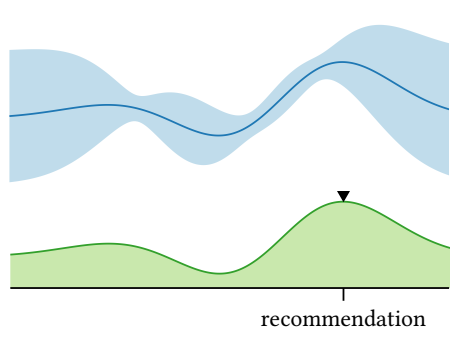
\includegraphics[width=0.4\linewidth]{figure/image1.png}
  \end{figure}  
\end{frame}

% 8 page
% 9 page
\section{Sequential Decisions with a Fixed Budget}
\begin{frame}{Sequential Decision}
  \begin{itemize}
    \item Isolated decision: an uncertainty r.v. $\psi$ would affect the action $a$, and therefore the outcome dataset.
    \item \textbf{Sequential decision}: whenever we make a decision, the updated dataset reduces the uncertainty about $\psi$.
    \item[$\Rightarrow$] We have to consider the updated observation $(x,y)$ as the one that would affect all future decisions.
    \vspace{1.0em}
    \item We will reason the final decision first, and define the optimization policy in reverse.
    \item \textbf{Fixed, known budget}: Assume that we have a fixed number of iterations $\tau$ to make decisions, and we want to maximize the expected utility of the final decision.
  \end{itemize}
\end{frame}

% 10 page
\begin{frame}
  At this time, for the dataset $\mathcal{D}$ and the decision horizon $\tau,$ let
  \[
    \begin{aligned}
      \mathcal{D}_1 &= \mathcal{D} \cup \{(x_1, y_1)\}, \\
      \mathcal{D}_2 &= \mathcal{D}_1 \cup \{(x_2, y_2)\}, \\
      &\vdots \\
      \mathcal{D}_\tau &= \mathcal{D}_{\tau-1} \cup \{(x_\tau, y_\tau)\}.
    \end{aligned}
  \]
  where $x_t$ is the point selected at step $t$ and $y_t$ is the observed value of the objective function at $x_t.$
  \vspace{1.0em}
  Then, our interest is the utility of the final dataset:
  \[
    u(\mathcal{D}_\tau)
    =
    u\big(
    \underbrace{\mathcal{D}}_{\text{known}},
    \underbrace{x}_{\text{action}},
    \underbrace{y, x_2, y_2, \ldots, x_\tau, y_\tau}_{\text{unknown}}
    \big),
  \]
  and the expected terminal utility:
  \[
    \mathbb{E}[u(\mathcal{D}_\tau) \mid x, \mathcal{D}] = \int u(\mathcal{D}_\tau) p(y \mid x, \mathcal{D}) \prod_{i=2}^\tau p(x_i, y_i \mid \mathcal{D}_{i-1}) dy d\{(x_i, y_i)\},
  \]
  or the expected increase in utility:
  \[
    \alpha_\tau(x; \mathcal{D}) = \mathbb{E}[u(\mathcal{D}_\tau) \mid x, \mathcal{D}] - u(\mathcal{D}).
  \]
\end{frame}

% 11 page
\begin{frame}{Case 1: One observation remaining ($\tau = 1$)}
  \begin{itemize}
    \item It is the same as the isolated decision case, and the optimal action is
    \[
      x \in \arg\max_{x' \in \mathcal{X}} \alpha_1(x'; \mathcal{D}) = \arg\max_{x' \in \mathcal{X}} \int u(\mathcal{D}_1) p(y \mid x', \mathcal{D}) dy - u(\mathcal{D}).
    \]
    and then the utility of the final dataset is
    \[
      u(\mathcal{D}_1) = u(\mathcal{D}) + \alpha_1^*(\mathcal{D})
    \]
    where $\alpha_1^*(\mathcal{D}) = \max_{x' \in \mathcal{X}} \alpha_1(x'; \mathcal{D}).$
  \end{itemize}
\end{frame}

% 12 page
\begin{frame}{Example: Intuitive Utility Function}
  \begin{itemize}
    \item $p(f \mid \mathcal{D})$ is a Gaussian process.
    \begin{figure}
        \centering
        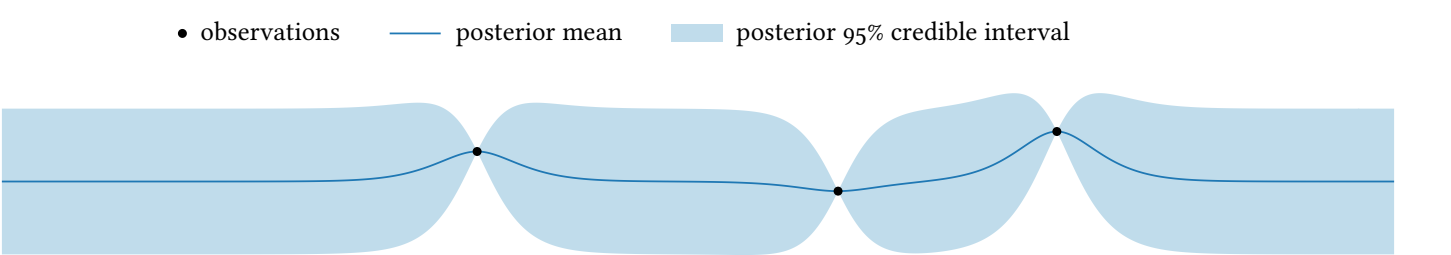
\includegraphics[width=\linewidth]{figure/image2.png}
    \end{figure}
    \item The utility function is naturally selected as the maximum value of the objective function:
    \[
      u(\mathcal{D}) = \max f(\bold x).
    \]
  \end{itemize}
\end{frame}

% 13 page
\begin{frame}
  \begin{itemize}
    \item[$\Rightarrow$] Then, the marginal gain in utility for the final observation $(x, y)$ is:
    \[
      u(\mathcal{D}_1) - u(\mathcal{D}) = \max\{y - u(\mathcal{D}), 0\}.
    \]
    \begin{figure}
        \centering
        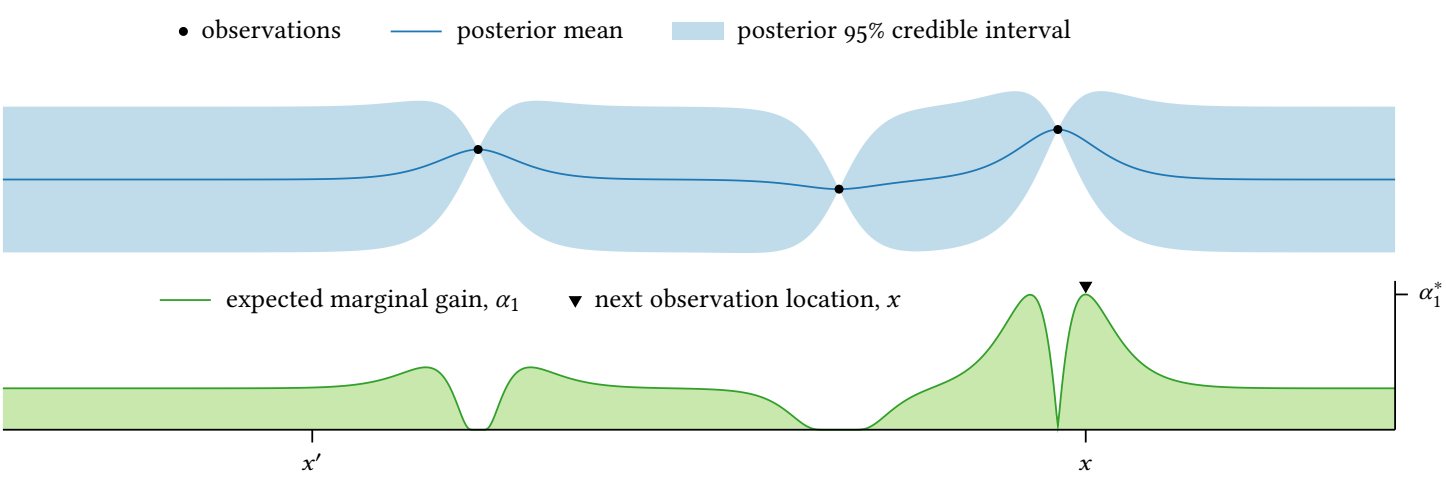
\includegraphics[width=\linewidth]{figure/image3.png}
    \end{figure}

    \begin{figure}
        \centering
        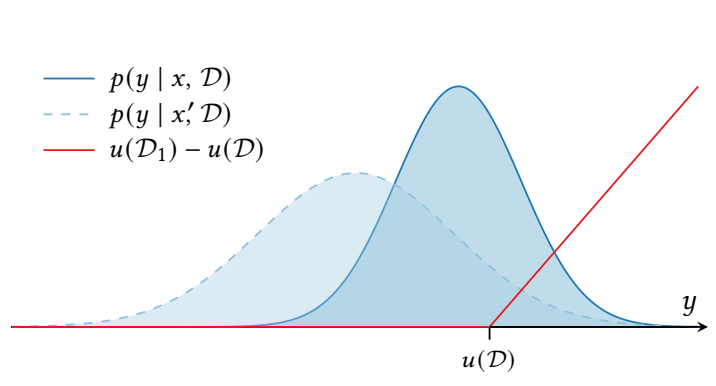
\includegraphics[width=0.5\linewidth]{figure/image4.png}
    \end{figure}
  \end{itemize}
\end{frame}

% 14 page
\begin{frame}{Case 2: Two observations remaining ($\tau =2)$}
  For the expected increase in utility $\alpha_2(x; \mathcal{D}) = \mathbb{E}[u(\mathcal{D}_2) \mid x, \mathcal{D}] - u(\mathcal{D}),$ we can decompose it as
  \[
    \begin{aligned}
      \alpha_2(x; \mathcal{D}) &= \mathbb{E}[u(\mathcal{D}_2) - u(\mathcal{D}) \mid x, \mathcal{D}]  \\
      &= \mathbb{E}[u(\mathcal{D}_2) - u(\mathcal{D}_1) + u(\mathcal{D}_1) - u(\mathcal{D}) \mid x, \mathcal{D}] \\
      &= \alpha_1(x; \mathcal{D}) + \mathbb{E}[ \mathbb{E}[u(\mathcal{D}_1) - u(\mathcal{D}) \mid x_2, \mathcal{D}_1] \mid x, \mathcal{D}] \\
      &= \underbrace{\alpha_1(x; \mathcal{D})}_{\text{immidiate gain}} + \underbrace{\mathbb{E}[\alpha_1(x_2; \mathcal{D}_1) \mid x, \mathcal{D}]}_{\text{future gain}}.
    \end{aligned}
  \]
  Now, assuming \textbf{optimal future behavior}, we have
  \[
    \alpha_2(x; \mathcal{D}) = \alpha_1(x; \mathcal{D}) + \mathbb{E}[\alpha_1^*(\mathcal{D}_1) \mid x, \mathcal{D}].
  \]
  which does not depend on the specific next action $x_2$, and its observation $y_2.$
\end{frame}

% 15 page
\begin{frame}{Example: Intuitive Utility Function}
  \begin{figure}
        \centering
        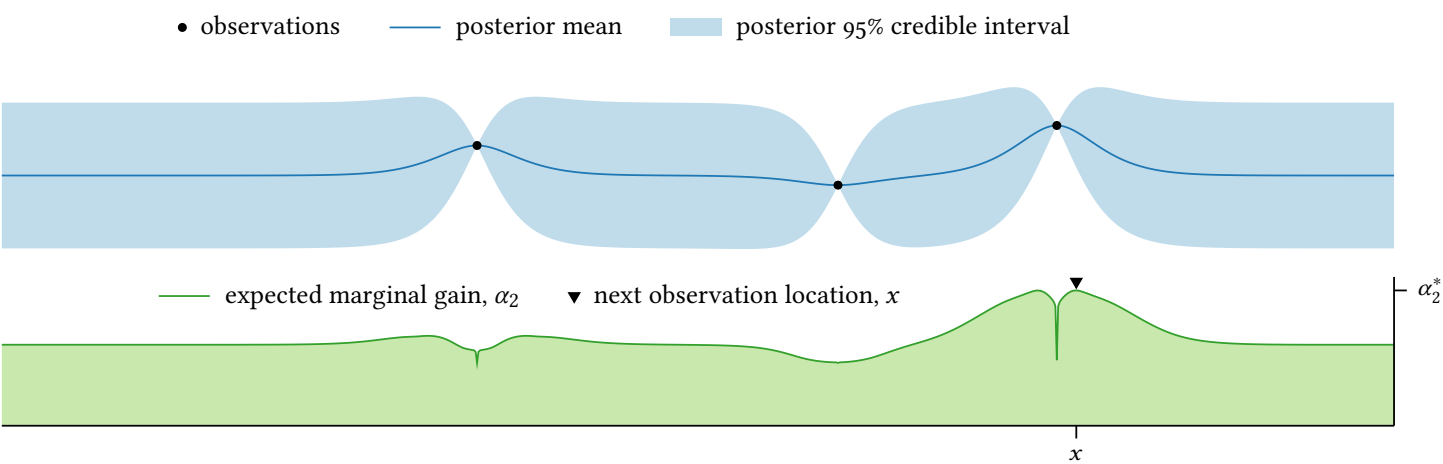
\includegraphics[width=0.6\linewidth]{figure/image5.png}
        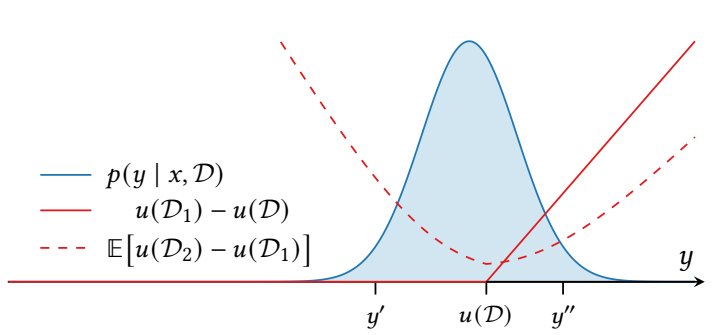
\includegraphics[width=0.38\linewidth]{figure/image6.png}
  \end{figure}
  \vspace{0.5em}
  \begin{figure}
        \centering
        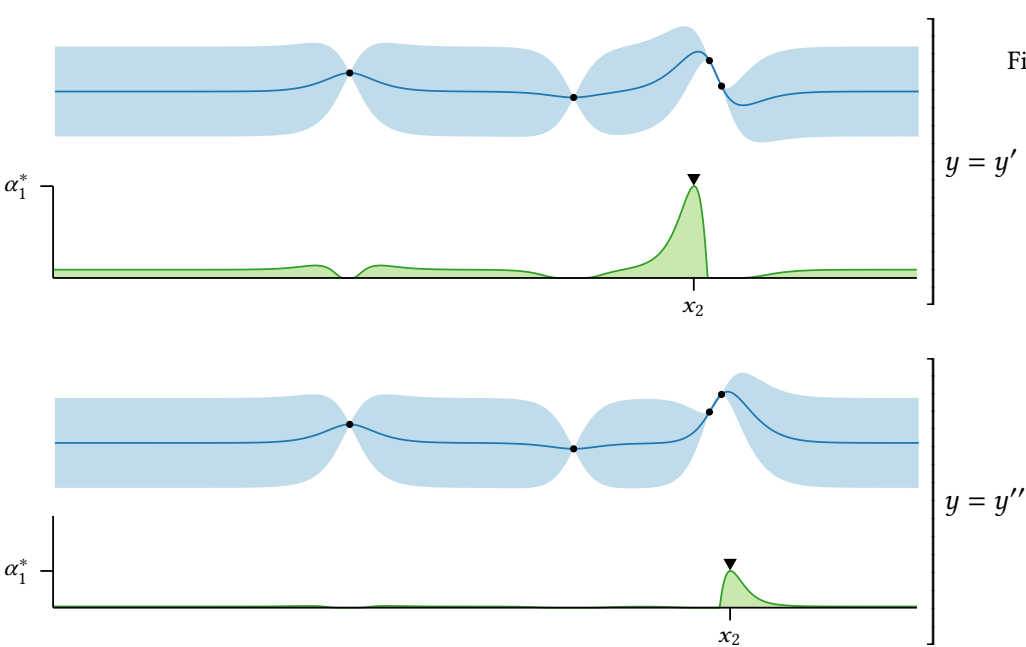
\includegraphics[width=0.6\linewidth]{figure/image7.png}
  \end{figure}
\end{frame}

% 16 page
\begin{frame}{Case 3: General case}
  Consider the $\tau$-step expected gain in utility $\alpha_\tau(x; \mathcal{D}) = \mathbb{E}[u(\mathcal{D}_\tau) \mid x, \mathcal{D}] - u(\mathcal{D}),$ which we seek to maximize. 
  It can be decomposed as the sum of the immediate gain and the expected future gain:
  \[
    \alpha_\tau(x; \mathcal{D}) = \alpha_1(x; \mathcal{D}) + \mathbb{E}[\alpha_{\tau-1}(x_2; \mathcal{D}_1) \mid x, \mathcal{D}].
  \]
  Also, by the assumption of optimal future behavior,
  \[
    \alpha_\tau(x; \mathcal{D}) = \alpha_1(x; \mathcal{D}) + \mathbb{E}[\alpha_{\tau-1}^*(\mathcal{D}_1) \mid x, \mathcal{D}].
  \]

  \begin{block}{Def: Bellman Equation for Optimal Sequential Decision}
    \[
      \begin{aligned}
        x &\in \arg\max_{x' \in \mathcal{X}} \alpha_\tau(x'; \mathcal{D}) \\
        &= \arg\max_{x' \in \mathcal{X}} \left\{\alpha_1(x'; \mathcal{D}) + \mathbb{E}[\alpha_{\tau-1}^*(\mathcal{D}_1) \mid x', \mathcal{D}]\right\},
      \end{aligned}
    \]
    and it is executed recursively until $\tau = 0,$ in this fixed-horizon setting.
  \end{block}
  Q. Summarize the Bellman equation and Bellman optimality.
  \newline
  A. Recursively evaluate (present reward + next value) going forward one step.
\end{frame}

% 17 page
% 18 page
\section{Cost and Approximation of the Optimal Policy}
\begin{frame}{High Cost of Ideal Sequential Decision-Making}
  \begin{figure}
        \centering
        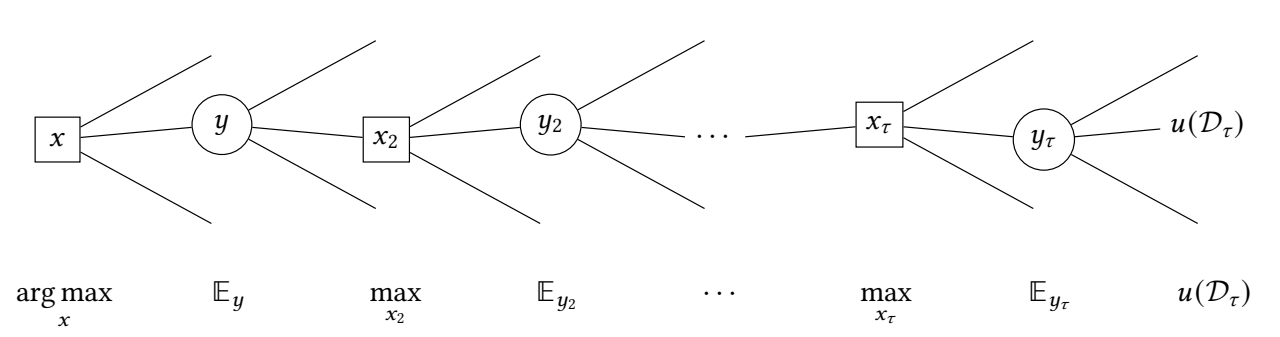
\includegraphics[width=0.9\linewidth]{figure/image8.png}
  \end{figure}
  Unrolling the optimal $\tau-$step optimization policy,
  \[
    \begin{aligned}
      x &\in \arg\max_{x' \in \mathcal{X}} \alpha_\tau (x', \mathcal{D}) \\
      &= \arg\max \left\{\alpha_1(x'; \mathcal{D}) + \mathbb{E}[\alpha_{\tau-1}^*(\mathcal{D}_1) \mid x', \mathcal{D}]\right\} \\
      &= \arg\max \left\{\alpha_1(x'; \mathcal{D}) + \mathbb{E}\left[\max_{x''}\alpha_1(x''; \mathcal{D}_1) + \mathbb{E}[\alpha_{\tau-2}^*(\mathcal{D}_2) \mid x'', \mathcal{D}_1] \mid x', \mathcal{D}\right] \right\} \\
      &= \cdots,
    \end{aligned}
  \]
  which is computationally intractable for large $\tau.$
\end{frame}

% 19 page
\begin{frame}
  \begin{itemize}
    \item $n$ evaluations of the objective for each call to the optimizer,
    \item and $q$ observations of the integrand for each call to the quadrature routine,
    \item[$\Rightarrow$] then, the total cost of computing $\alpha_\tau(x; \mathcal{D})$ is
    \[
      \mathcal{O}(n^\tau q^\tau).
    \]
  \end{itemize}
  \vspace{2.0em}
  Then, for the intractable optimal expected marginal gain 
  \[
    \alpha_\tau(x; \mathcal{D}) = \alpha_1(x; \mathcal{D}) + \mathbb{E}[\alpha_{\tau-1}^*(\mathcal{D}_1) \mid x, \mathcal{D}],
  \] 
  we have to approximate its second term by some computationally tractable surrogate.
  \begin{itemize}
    \item Limited lookahead
    \item Rollout
  \end{itemize}
\end{frame}

% 20 page
\begin{frame}{Approximation of the Optimal Policy: Limited Lookahead}
  \begin{itemize}
    \item Decisions closer to termination require substantially less computation than earlier decisions.
    \item If we expect decreasing marginal gains, implying a significant fraction of potential gains can be attained within the truncated horizon.
    \item[$\Rightarrow$] \textbf{$\ell-$step lookahead policy}: Truncate the expected future gain after $\ell$ steps, 
    and use the optimal $\ell-$step policy as a surrogate for the optimal $\tau-$step policy.
    \newline
    \item Since an infeasible decision horizon $\tau$ is considered as
    \[
      \alpha_\tau(x; \mathcal{D}) \approx \alpha_\ell(x; \mathcal{D}),
    \]
    each observation requires to maximize the acquisition function
    \[
      \alpha_{\min\{\ell, \tau\}}(x; \mathcal{D}) = \alpha_1(x; \mathcal{D}) + \mathbb{E}[\alpha_{\min\{\ell-1, \tau-1\}}^*(\mathcal{D}_1) \mid x, \mathcal{D}].
    \] 
    \item The computational cost is bounded at most by $\mathcal{O}(n^\ell q^\ell)$.
  \end{itemize}
\end{frame}

% 21 page
\begin{frame}{Additional Considerations in Limited Lookahead}
  \textbf{One-step lookahead ($\ell = 1$)}
  \begin{itemize}
    \item Only consider a single additional observation, $\alpha_1$, and then the policy is quite myopic.
    \item It is often possible to derive a closed-form, which is analytically differentiable for $\alpha_1$.
    \item (Chapter 7) Many well-known acquisition functions represent
    one-step lookahead approximations for some implicit choice of utility function.
  \end{itemize}

  \[
    \begin{aligned}
      x &\in \arg\max_{x' \in \mathcal{X}} \alpha_1(x'; \mathcal{D}) \\
      &= \arg\max_{x' \in \mathcal{X}} \mathbb{E}_{y \sim p(y \mid x', \mathcal{D})}[u(\mathcal{D}_1) - u(\mathcal{D}) \mid x', \mathcal{D}].
    \end{aligned}
  \]
  \vspace{1.0em}
  \small{\begin{itemize}
    \item[Q.] How to choose $\ell$?
    \item[A.] By the cost-benefit tradeoff, it can be determined by the computational budget and the expected marginal gain of additional lookahead.
    \item[Ex.] (1) 2-step lookahead: \cite{wu2019practical, zhang2021constrained}
    \item[] (2) \cite{byun2022multi}
    \begin{figure}
        \centering
        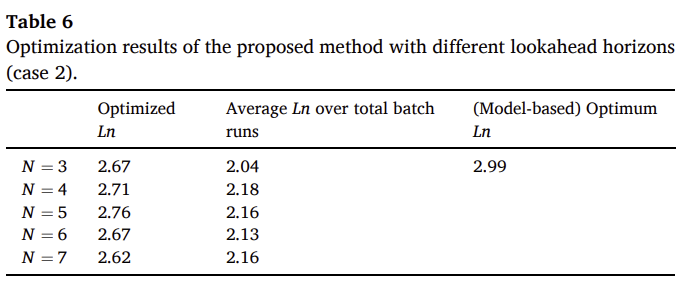
\includegraphics[width=0.4\linewidth]{figure/cite1.png}
    \end{figure}
  \end{itemize}}
\end{frame}

% 22 page
\begin{frame}{Approximation of the Optimal Policy: Rollout}
  \begin{figure}
        \centering
        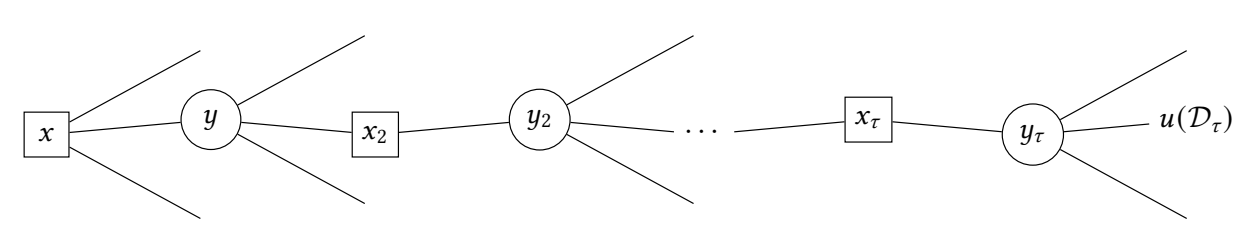
\includegraphics[width=0.9\linewidth]{figure/image9.png}
  \end{figure}
  \textbf{Rollout}
  \begin{itemize}
    \item Given a next putative observation $(x, y)$, for the following decisions $x_2,$ we use a base (or heuristic) policy that is a
    \begin{itemize}
      \item inexpensive,
      \item plausible, and
      \item perhaps suboptimal
    \end{itemize}
    simulation.
    \vspace{0.7em}
    \item There are no constraints on the design of the base policy, but for the success of the approximation, 
    we must choose something relatively efficient.
  \end{itemize}
  
\end{frame}

% 23 page
\begin{frame}{Rollout with one-step lookahead}
  \begin{itemize}
    \item The base policy is the one-step lookahead policy, i.e., we do simulate future decisions with the one-step lookahead policy.
    \item Then,
    \begin{exampleblock}{Rollout with one-step lookahead}
      \begin{enumerate}
        \item Fix the candidate $x'.$ ($n$ evaluations)
        \item For each candidate, sample $q$ observations $y \sim p(y \mid x', \mathcal{D}).$
        \begin{enumerate}
          \item For each y, apply the one-step lookahead policy:
          \[
            x_2 \in \arg\max_{x' \in \mathcal{X}} \alpha_1(x'; \mathcal{D}_1).
          \] 
          \item Sample $q$ obs., one-step $x_3$, and so on.
        \end{enumerate}
        \item[$\Rightarrow$] $\mathcal{O}(n^2 q^\tau)$ (and typically $q << n.$)
      \end{enumerate}
    \end{exampleblock}
  \end{itemize}
  Q. Why is the cost $\mathcal{O}(n^2 q^\tau)$?
  \newline
  A.
\end{frame}

% 24 page
\begin{frame}{Additional Considerations in Rollout}
  \textbf{$\ell$-step lookahead}
  \begin{itemize}
    \item Base policy: the next $\ell-1$ decisions are selected optimally,
    \item and then simply terminate early, even if the budget is not exhausted.
    \item[$\Rightarrow$] $\mathcal{O}(n^\ell q^\ell)$ 
  \end{itemize}
  
  \vspace{1.0em}
  \textbf{Batch rollout}
  \begin{itemize}
    \item Base policy: all remaining decisions are selected simultaneously.
    \item[$\Rightarrow$] $\mathcal{O}(n q^\tau)$
  \end{itemize}
\end{frame}

% 25 page
\section{Cost-Aware Optimization and Termination as a Decision}
\begin{frame}{Dynamic Termination}
  \begin{itemize}
    \item Fixed, known budget scenario is pervasive, but not universal.
    \item Instead, we want to use the future belief about the objective functions to decide dynamically when to stop the optimization process.
    \item Especially, if the cost of data acquisition were to vary across the domain, it would be weird to define a fixed budget.
    \vspace{1.0em}
    \item Idea: \textbf{Account for observation costs in the utility function.}
    \item[$\Rightarrow$] Then, the cost-benefit tradeoff allows us naturally to decide when to terminate it.
  \end{itemize}
\end{frame}

% 26 page
\begin{frame}{Model Termination Decision}
  We consider a modification to the sequential decision problem we analyzed in the known-budget case.
  \begin{itemize}
    \item Extension of the action space $\mathcal{A}:$
    \[
      \mathcal{A} = \mathcal{X} \cup \{\emptyset\},
    \]
    \item Once the termination action $\emptyset$ is selected, the decision process continues with the collapsed action space $\mathcal{A} = \{\emptyset\}$
    \item[$\Rightarrow$] Then, we can consider this as the fixed, known budget case.
    \vspace{1.0em}
    \item On the decision horizon $\tau,$ we execute the induction step from the final decision, but in this adaptive termination case, 
    the observation can be selected infinitely many times.
    \item[$\Rightarrow$] To sidestep this issue, we can simply assume that the upper bound $\tau_\text{max}$ on the total number of observations. 
    (not an overly restrictive assumption)
  \end{itemize}
\end{frame}

% 27 page
\begin{frame}
  \begin{itemize}
    \item Since 
    \[
      \alpha_\tau(\emptyset; \mathcal{D}) = 0,
    \]
    the optimal termination policy is given by
    \[
      \alpha_\tau^*(\mathcal{D}) = 0.
    \]
    \item But, most of the utility functions we have considered are probably always positive,
    since the information has a small amount of value, no matter how useless it may be.
    \item[$\Rightarrow$] \textbf{Cost-aware optimization}
  \end{itemize}
\end{frame}

% 28 page
\begin{frame}{Cost-aware Optimization}
  \begin{itemize}
    \item Data utility
    \[
      u'(\mathcal{D}).
    \]
    \item Cost function (additive in many cases)
    \[
      c(\mathcal{D}) = \sum_{x \in \mathcal{D}} c(x).
    \]
    \item Cost-adjusted utility
    \[
      u(\mathcal{D}) = u'(\mathcal{D}) - c(\mathcal{D}).
    \]
  \end{itemize}
\end{frame}

% 30 page
\begin{frame}{Example: one-step lookahead with cost-aware utility}
  \begin{itemize}
    \item cost-unaware policy:
    \[
      x \in \arg\max_{x' \in \mathcal{X}} \alpha_1'(x'; \mathcal{D}) = \arg\max_{x' \in \mathcal{X}} \mathbb{E}_y[u'(\mathcal{D}_1)-u'(\mathcal{D}) \mid x', \mathcal{D}].
    \]
    \item cost-aware policy:
    \[
      x \in \arg\max_{x' \in \mathcal{X}} \alpha_1(x'; \mathcal{D}) = \arg\max_{x' \in \mathcal{X}} \mathbb{E}_y[u(\mathcal{D}_1) - u(\mathcal{D}) \mid x', \mathcal{D}] - c(x').
    \]
  \end{itemize}
  \begin{figure}
        \centering
        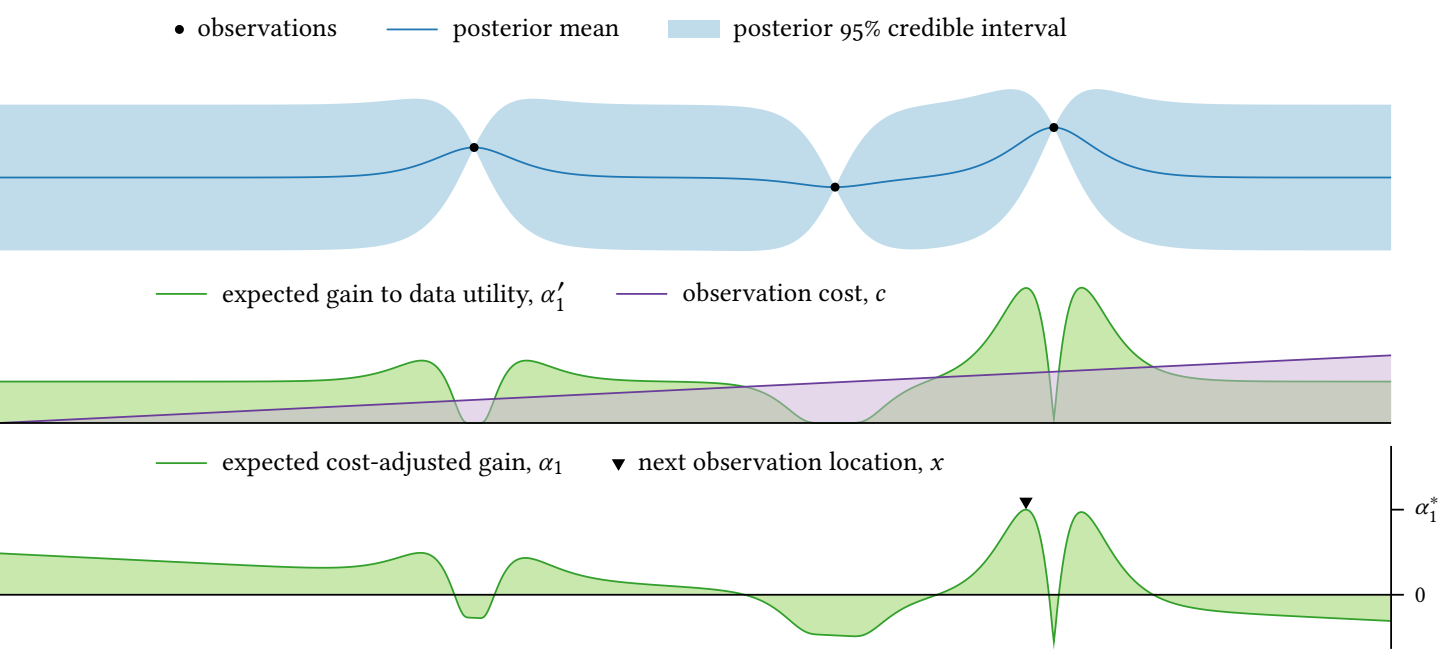
\includegraphics[width=0.7\linewidth]{figure/image10.png}
  \end{figure}
  \small{Q. What means the cost-adjusted expected gain is negative?
  \newline
  A. (1) gain < cost, (2) still gain is positive, (3) but the termination is when $\max \alpha_1 \le 0.$}
\end{frame}

% 31 page
\begin{frame}{Questions}
  Q. Is it really efficient to use the optimal $\ell$-step lookahead policy as a surrogate for the optimal $\tau$-step policy?
  \newline
  A. First, the optimal limited lookahead policy is equivalent to the multi-step rollout policy.
  \begin{alertblock}{Prop. 2.4. in \cite{bertsekas2025neuro}}
    The policy iteration algorithm generates an improving sequence of proper polices,
    [that is, $J^{\mu_{k+1}}(i) \le J^{\mu_k}(i)$ for all $i$ and $k$] and terminates with an optimal policy.
  \end{alertblock}
\end{frame}

% 32 page
\begin{frame}
  Q. Is there any way to quantify the optimization performance of the selected policy? If so, does it depend on the decision horizon $\tau$?
  \newline
  A. (Chapter 10) \textbf{Regret analysis.}
  \begin{itemize}
    \item \textbf{Simple regret} at time $\tau$ is the difference between the optimal value of the objective function 
    and the value of the best point observed up to time $\tau.$
    \[
      r_\tau = \max_{x \in \mathcal{X}} f(x) - \max_{(x, y) \in \mathcal{D}_\tau} y,
    \]
    \item \textbf{Cumulative regret} at time $\tau$ is the sum of the differences between the optimal value of the objective function 
    and the value of the point selected at each time step up to time $\tau.$
    \[
      R_\tau = \sum_{i=1}^\tau \left(\max_{x \in \mathcal{X}} f(x) - f(x_i)\right).
    \]
    \item Since $r_\tau \le \frac{R_\tau}{\tau}$, our goal is the no-regret property of the optimization policy, i.e.,
    \[
      \lim_{\tau \to \infty} \frac{R_\tau}{\tau} = 0.
    \]
    \item[$\Rightarrow$] In RKHS ($\because$ continuous function space is too large ), by GP-UCB, for a smooth Gaussian proc. s.p. with Matern family,
    \[
      R_\tau = \mathcal{O}^*(\sqrt{\tau (\log \tau)^d}).
    \]
  \end{itemize}
\end{frame}

% 33 page
\begin{frame}
  Q. (Chapter 11.1.) How about the case of an unknown observation cost?
  \newline
  A. If the observation cost were only determined through the course of acquisition, we have to consider the inference about observation costs throughout optimization,
  and use the posterior belief about the cost to make decisions.
  \begin{itemize}
    \item For an underlying cost function $c: \mathcal{X} \rightarrow \mathbb{R},$ assume that
    the evaluation at $x$ returns both 
    \begin{itemize}
      \item a measured value $y$ whose distribution depends on the objective function $\psi = f(x),$
      \item and an observation cost $z$ whose distribution depends on the cost function $\kappa = c(x).$
    \end{itemize}
    \item[$\Rightarrow$] Then, for the inference of the posterior distribution about the cost $p(c \mid \mathcal{D}),$
    we can obtain the predictive distribution of the cost
    \[
      p(z \mid x, \mathcal{D}) = \int p(z \mid x, \kappa) p(\kappa \mid x, \mathcal{D}) d\kappa,
    \]
    and hence the expected cost-adjusted gain in utility is
    \[
      \begin{aligned}
        \alpha_1(x; \mathcal{D}) &= \mathcal{E}_{y,z \sim p(y,z \mid x, \mathcal{D})}[u(\mathcal{D} \cup \{(x, y, z)\}) - u(\mathcal{D})]\\
        &= \int \int (u(\mathcal{D}_1) - u(\mathcal{D}) - c(z)) p(y \mid x, \mathcal{D}) p(z \mid x, \mathcal{D}) dy dz,
      \end{aligned}
    \]
    especially if the cost is additive.
  \end{itemize} 
\end{frame}

% =========================
\begin{frame}[allowframebreaks]{References}
\footnotesize
\bibliographystyle{plain}
\bibliography{references}
\end{frame}

\end{document}